\documentclass{beamer}
\usetheme{}
\title{Using occupancy theory and Bayesian models to estimate otter populations in southeastern Minnesota}
\author[Aing, Halls, Oken]{Chrisna Aing, Sarah Halls, Kiva Oken}
\institute{Carleton College}
\usepackage{graphpap,graphics}
%\includeonlyframes{}

\begin{document}
	{
	\usebackgroundtemplate{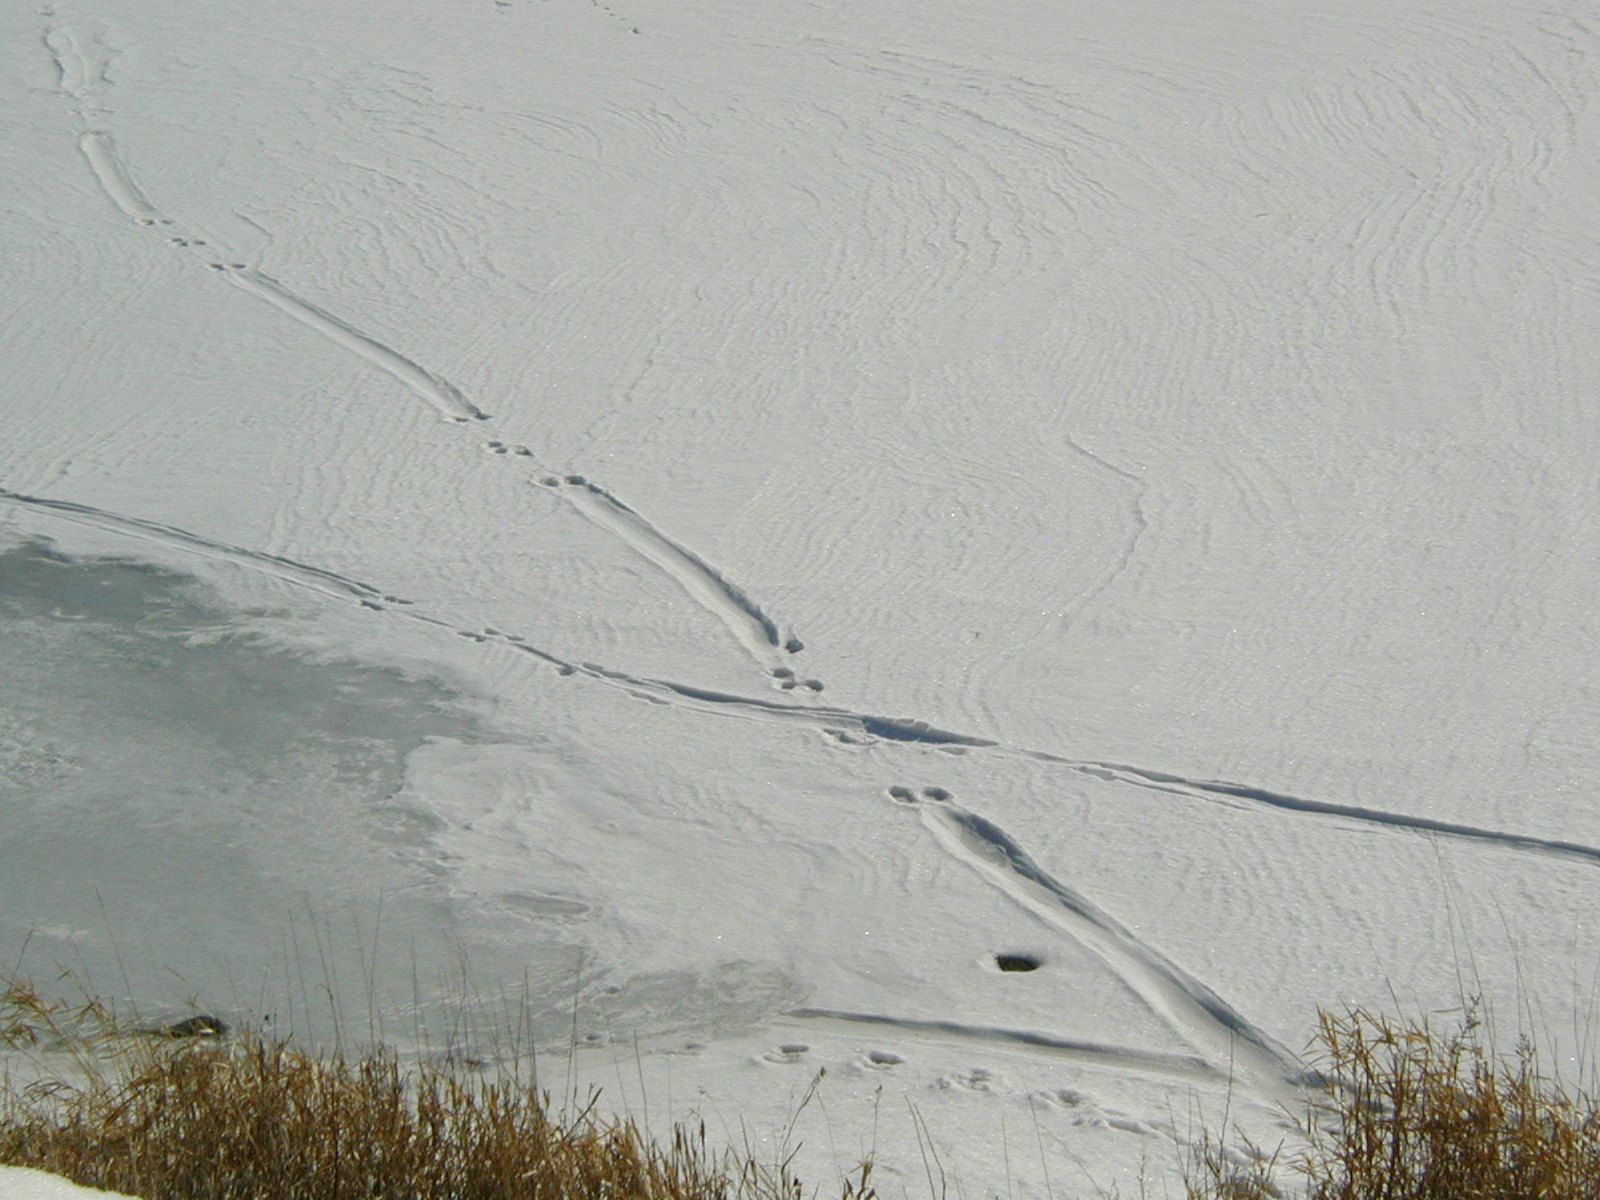
\includegraphics[width=\paperwidth]{ottertracks1.jpg}}

\begin{frame}
	\titlepage
\end{frame}
}
\begin{frame}
	\tableofcontents[pausesections]
\end{frame}

\section{The data and questions}
\begin{frame}{Otters}
	\begin{columns}
		\column{5cm}
		\begin{itemize}[<+->]
			\item Otters endemic to all of Minnesota
			\item Indicator species for quality of aquatic habitat
			\item Populations crashed, now rebounding
			\item In SE Minnesota interest in resuming trapping
			\item Government needs tools to monitor changes in populations
		\end{itemize}
		\column{5cm}
		\resizebox{5cm}{!}{\includegraphics{cuteOtter1.pdf}}
	\end{columns}
\end{frame}

\begin{frame}{Collecting data}
	\begin{columns}
		\column{5cm}
		\resizebox{5cm}{!}{\includegraphics{cuteOtter1.pdf}}
		\column{5cm}
		\begin{itemize}[<+->]
			\item Researchers flew over rivers during winters of 2003, 2004
			\item Flew one, two, or three days after snow events
			\item Marked GPS coordinates of tracks
			\item Rivers divided into 400, 800, or 1600 m plots
			\item Presence of track in each plot determined
		\end{itemize}
	\end{columns}
\end{frame}

{
	\usebackgroundtemplate{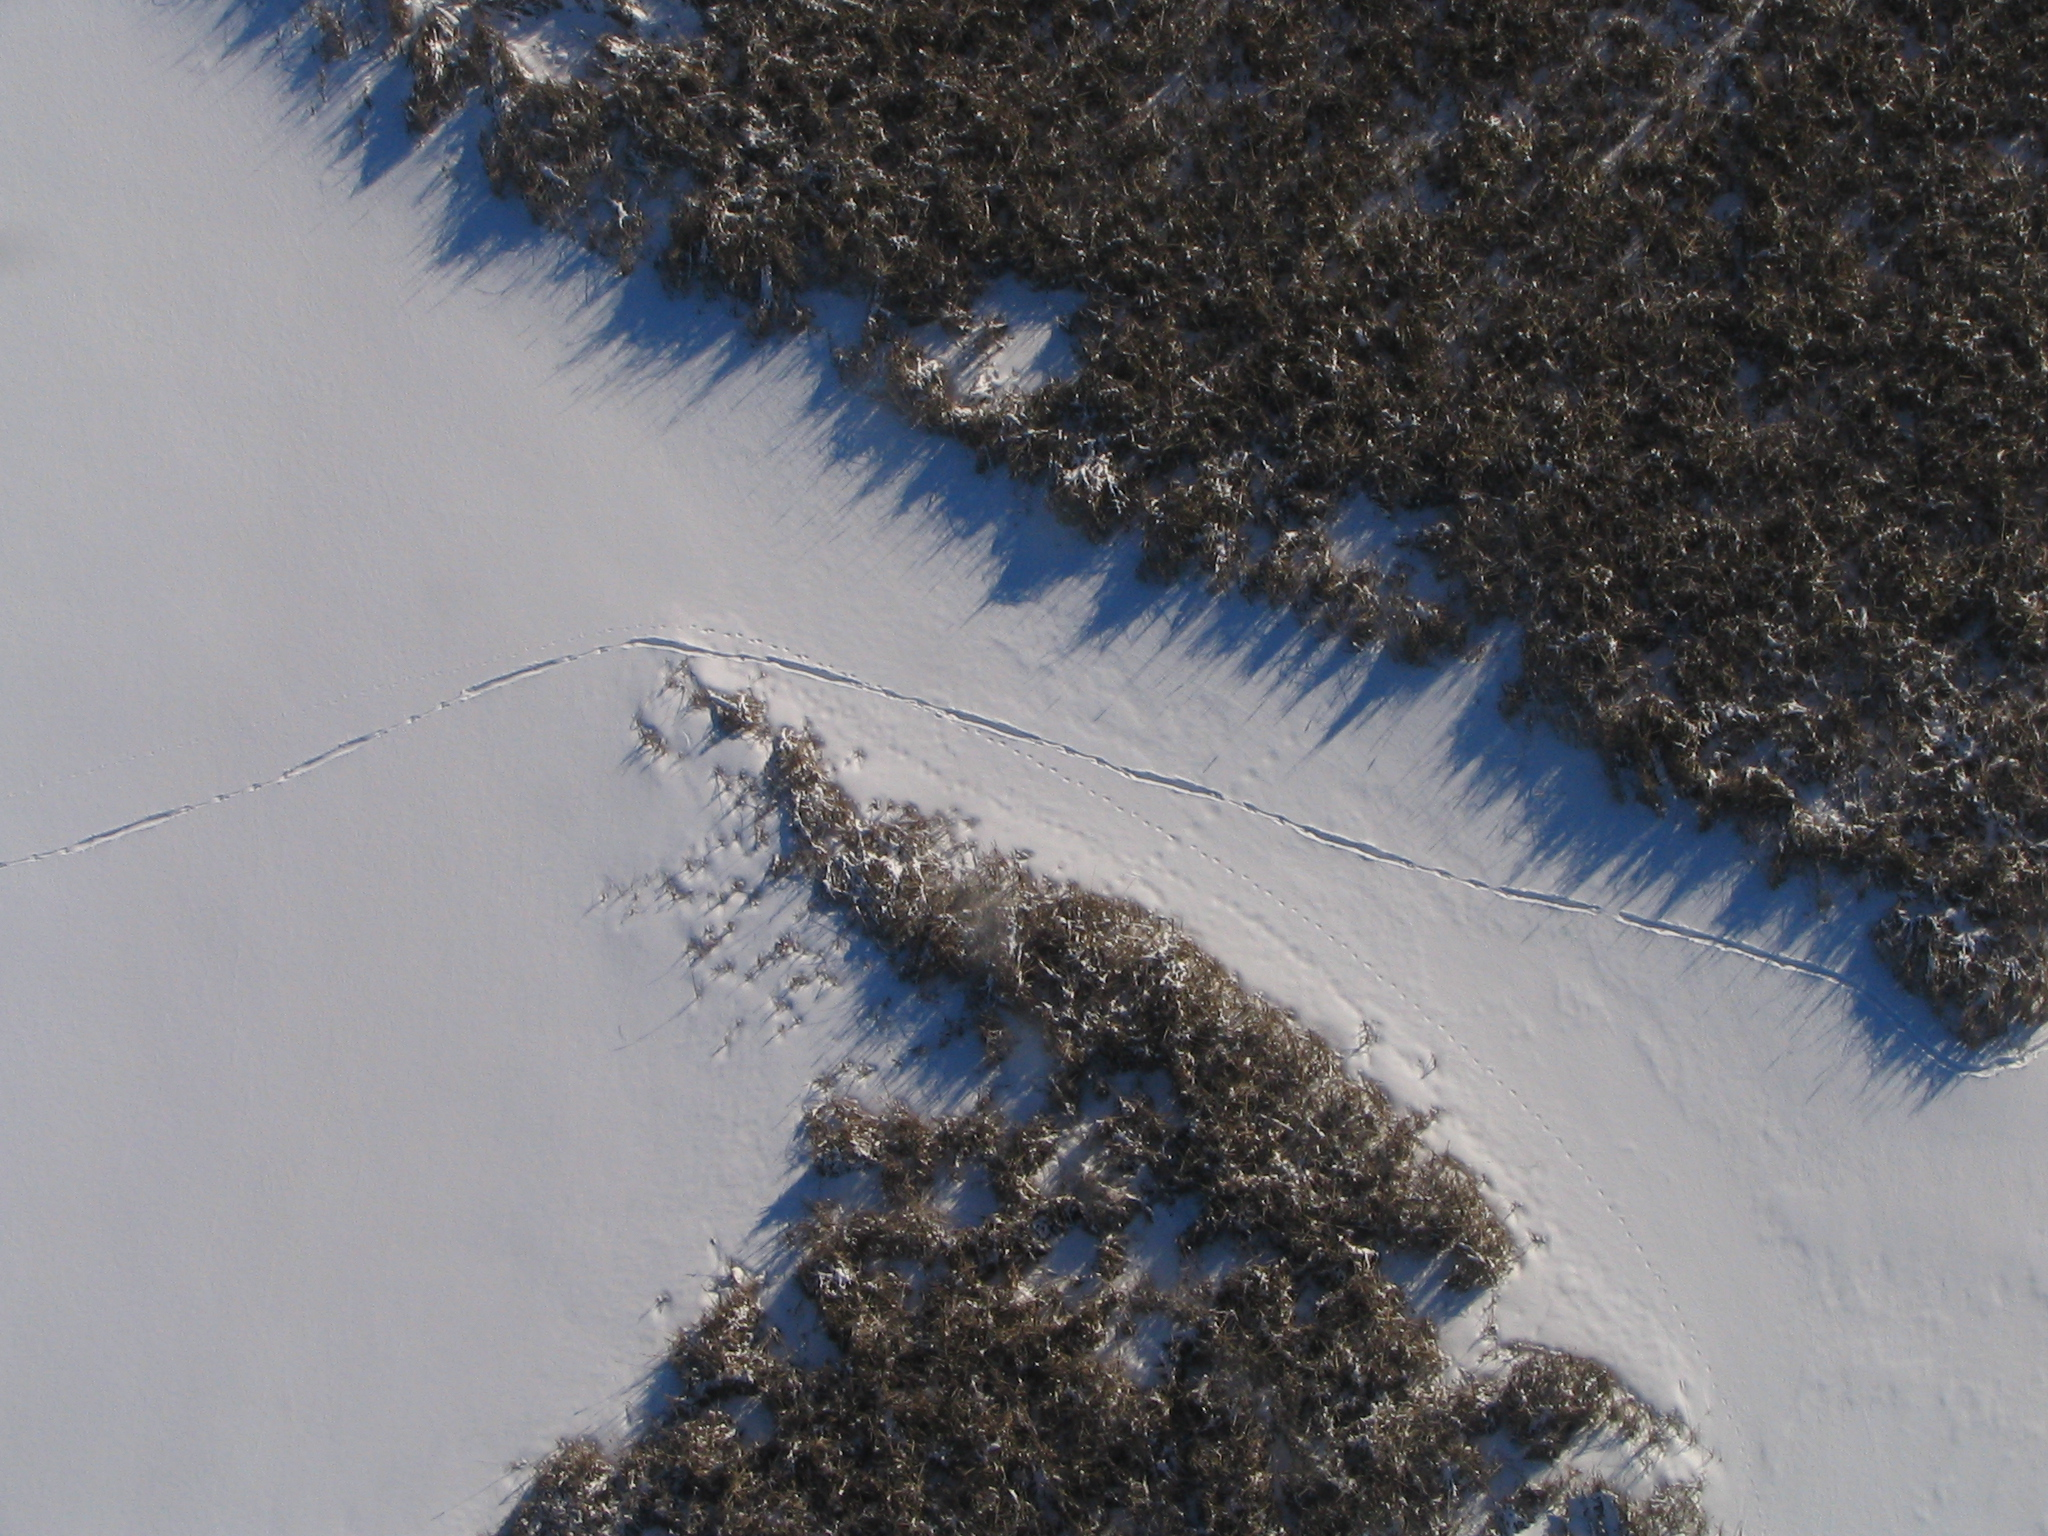
\includegraphics[width=\paperwidth]{SnowTracks12.jpg}}
	\begin{frame}{}
	\end{frame}
}

{
	\usebackgroundtemplate{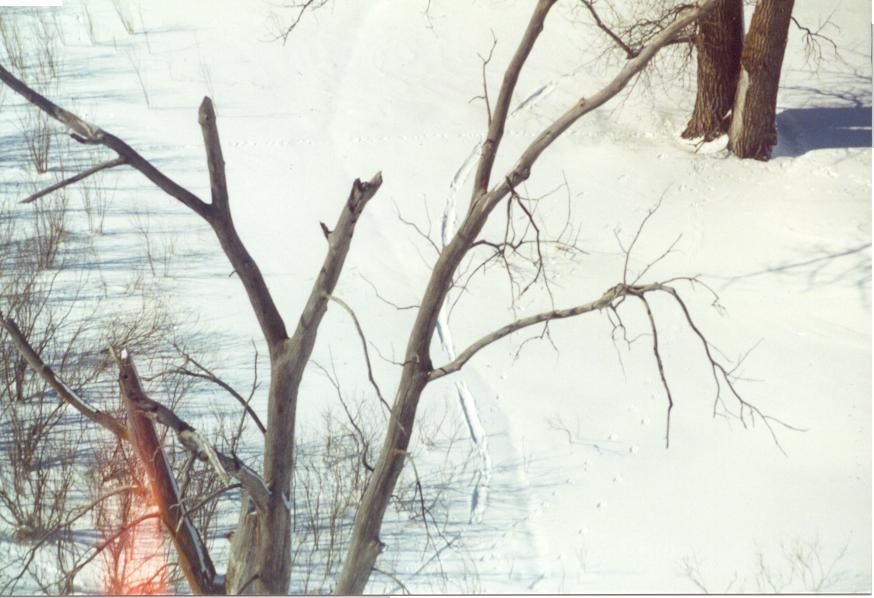
\includegraphics[width=\paperwidth]{SNOWTRACKS9.jpg}}
	\begin{frame}
	\end{frame}
}

\begin{frame}{Issues related to data}
	\begin{itemize}
		\item Tracks near plot boundary can be assigned to different plots
		\item Track in one site means more likely to be track in neighboring site- not independent
	\end{itemize}
\end{frame}

\section{Occupancy Theory}
\begin{frame}{Definitions of occupancy}
	\begin{itemize}
		\item The probability that a randomly selected site or sampling unit in an area of interest is occupied by a species
		\item The proportion of area, patches, or sampling units that is occupied 	\end{itemize}
	(MacKenzie, et al. 2006) 
\end{frame}

\begin{frame}{Estimating occupancy}
	\begin{itemize}
		\item Ecologists often conduct surveys to find the occupancy rate
		\item Not observing the species can mean two things:
		\begin{itemize}
			\item The species does not occupy the area
			\item The species went undetected during surveying
		\end{itemize}
		\item Need to be able to estimate probability of observing the species given its presence
	\end{itemize}
\end{frame}

\begin{frame}{Assumptions of occupancy models}
	\begin{itemize}
		\item No false positives
		\item Presence and detection probabilities are constant across sites and surveys (or can be modeled by covariates)
		\item Independence of detection between sites
		\item Survey is conducted on a closed population	\end{itemize}
\end{frame}

\begin{frame}{Types of occupancy models}
	\begin{itemize}
		\item Single species, single season
		\item Na\"ive occupancy: proportion of sites found to be occupied
		\item Hierarchical models
	\end{itemize}
	\begin{center}
		\resizebox{7cm}{!}{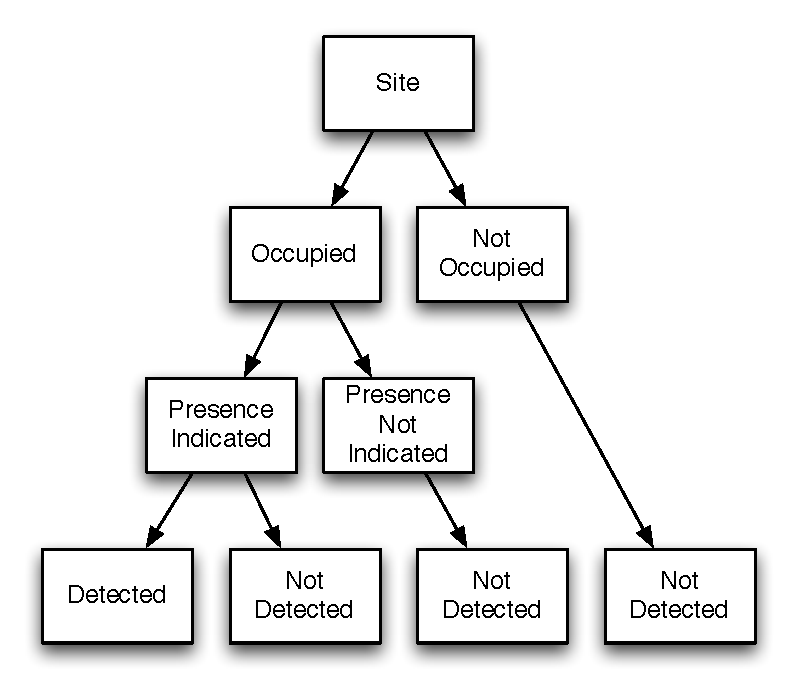
\includegraphics{SimpleHierarchicalModel.pdf}}
	\end{center}
\end{frame}

\begin{frame}{Parameters}
	\begin{itemize}
		\item $\psi=$ The probability a track is occupied
		\item $\theta=$ The probability a track is laid down in a site on a given day, given that the site is occupied
		\item $p= $ The probability an observer sees a track given that a track has been made
	\end{itemize}
\end{frame}

\section{Exploring the data}
\begin{frame}{Effects of multiple observers}
	\begin{itemize}
		\item In 2003, three different observers
		\item Detection rates varied among the observers
		%include graph here
		\item Solution: use observer indicators as covariates for detection probability
	\end{itemize}
\end{frame}

\begin{frame}{Correlation between flights}
	\begin{itemize}
		\item Two observers on same day should have the same na\"ive occupancy rates; not the case
		\item Also looked at correlation between flights
		\begin{itemize}
			\item Very low, overall
			\item Slightly higher during the same snow event or day
		\end{itemize}
		\item Solution: include false detection in model
	\end{itemize}
\end{frame}

%Include frame with new hierarchical diagram

\begin{frame}{Independence between plots}
	\begin{itemize}
		\item Assumption: independence between plots
		\item %Sarah going to review
		\item Solution: kept issue in mind, explored spatially explicit models
	\end{itemize}
\end{frame}

\section{Modeling the data}
\begin{frame}{Bayesian statistics}
\end{frame}

\begin{frame}{Our model}
\end{frame}

\begin{frame}{Testing the model- data simulations}
\end{frame}

\begin{frame}{Modeling spatial correlation}
\end{frame}

\begin{frame}{Testing the CAR model}
\end{frame}

\section{Discussion}
\begin{

\end{document}